\section{System overview}

The project will be set up as three main modules: Unreal Engine, AirSim and the fisheye camera. These are all compilable as their own packages, and does not need to be compiled in any specific order. Only Unreal Engine is executable on its own. AirSim is indirectly run by AirSim through adding the plugin to a specific unreal project, while the AirSim enabled project needs to be running within Unreal Engine in order to run or use the fisheye module. 

The AirSim plugin is made in a way, so that it technically resides outside of Unreal Engine. However it has full access to the resources of the Engine, through the engine's header files. Their design choice involves adding as much functionallity as possible, outside of the Engine, to make it easier to support other game engines, with only small changes to the AirSim package. The added features in the AirSim package includes: Multirotor and car models, perspective and depth camera, Lidar, IMU with magnetometer and GPS. In addition to this it supports HITL through the PX4 flight controller and MAVlink. 

As of now, AirSim is only usable with version 4.18 of Unreal Engine, while 4.21 is available at the time of writing. In order to reduce the chances of new commits to the original repositories causing problems for my project. Both AirSim and Unreal Engine4.18 have been forked to my own github. This allows me to control when to add the updates to the original projects, while enabling me to alter the packages as I choose. As of now Unreal Engine, and the project are made private due to licencing. However, my own alterations to AirSim are available publicly.

\subsection{Communication pattern}

Because of the design choices of AirSim, much of the simulator computations happen outside of Unreal Engine. While Unreal Engine handles the core game loop, resource management and the graphical tasks, custom AirSim scripts handle sensor simulation and kinematics. Of course, AirSim also relies on Unreal Engine for camera data, actor positions and pose, in addition to timing data. The AirSim plugin implements a game mode, which is run by Unreal Engine on simulation start. This decides whether to do a multirotor simulation, car simulation or computer vision mode. The computer vision mode turns off physics, enabling free camera movement for creating datasets. The game mode also sets up the program loop run for each actor each frame.

The API AirSim provides consists of a server/client based system, using the RPC\footnote{https://github.com/rpclib/rpclib} library. This enables messages to be sent over TCP/IP and allows making interfaces for multiple programming languages. The server is written in C++, and the client side is implemented for both Python and C++. As long as the server is enabled in the configuration file, it is started by Unreal Engine on simulation startup. 

\begin{figure}[!htb]
    \centering
    \begin{tikzpicture}[node distance=2.2cm, transform shape, scale=0.7]
        \tikzstyle{topblob} = [ellipse, minimum width = 7cm, minimum height = 2cm, text centered, draw=black, fill=blue!10]
        \tikzstyle{blob} = [ellipse, minimum width = 3cm, minimum height = 1.5cm, text centered, draw=black, fill=red!20]
        \tikzstyle{emphblob} = [ellipse, minimum width = 3cm, minimum height = 1.5cm, text centered, draw=black, fill=red!50]
        \tikzstyle{ownblob} = [ellipse, minimum width = 3cm, minimum height = 1.5cm, text centered, draw=black, fill=green!10]
        \tikzstyle{doublearrow} = [thick, <->, >=stealth]
        \tikzstyle{tcp} = [dashed]
        
        \node (UE) [topblob]{Unreal Engine};
        \node (AirSim) [blob, below of=UE, align=center, yshift=-0.5cm]{AirSim \\ Plugin Core};
        \node (Sens) [blob, left of=AirSim, align=center, xshift=-3cm]{Sensor \\ Models};
        \node (Phys) [blob, below right of=AirSim, align=center, xshift=3cm]{Physics \\ Engine};
        \node (cam) [emphblob, above of=Phys, align=center, yshift=0.5cm]{\textbf{Camera} \\ \textbf{Interface}};
        \node (RPCS) [blob, below of=AirSim]{RPC Server};
        \node (RPCC) [blob, below of=RPCS]{RPC Client};
        \node (Client) [ownblob, below of=RPCC]{ROS Client};
        \node (Fish) [ownblob, right of=RPCC, xshift=3cm, align=center]{Fisheye \\ Transform};
        
        \draw[doublearrow] (UE) -- (AirSim);
        \draw[doublearrow] (UE) -- (Sens);
        \draw[doublearrow] (UE) -- (cam);
        \draw[doublearrow] (AirSim) -- (Phys);
        \draw[doublearrow] (AirSim) -- (cam);
        \draw[doublearrow] (AirSim) -- (Sens);
        \draw[doublearrow] (AirSim) -- (RPCS);
        \draw[tcp] (RPCS) -- (RPCC); \node (tcpText) [left of=RPCC, , xshift=1cm, yshift=1.1cm]{\scriptsize TCP/IP};
        \draw[doublearrow] (RPCC) -- (Client);
        \draw[doublearrow] (Client) -- (Fish);
        
    \end{tikzpicture}
    \caption{Communication pattern of the fisheye camera simulator. Red nodes belong to the AirSim plugin, while Green nodes are custom made for this project. The emphasized node represent modified AirSim code.}
    \label{fig:comm_pattern}
\end{figure}

My project will be implemented for the multirotor game mode. This means that it will not run on the other game modes. The reason for this is that the cameras need to be setup specifically for each game mode, through the Unreal Engine Blueprints imported by the game mode. The fisheye camera and ROS interface will depend on the C++ RPC client API, the perspective camera model and the image capture module for AirSim. The contribution of my project will be to combine perspective images into a single fisheye lens distorted image, with as few changes as possible to the AirSim plugin. In addition to this I will build upon the C++ API to allow for publishing images to ROS, through the normal ROS publisher interface. Figure~\ref{fig:comm_pattern} shows the main communication flow of Unreal Engine, AirSim and the fisheye camera. As the project does not invole HITL with PX4, Mavlink or any controller setup, they are not shown in the Figure, and will not be discussed in this report.

\section{Implementation}

A couple of things to consider when implementing the fisheye camera is performance, maintainability, extendability, complexity and the timeframe to implement it. As this is done by one person in only a few months, the timeframe is the most important one. While maintainability and extendability are important factors, especially if this is to be distributed and used by others, the main goal is to get it working. However, both the ROS interface and the fisheye camera will be made as individual components, and should not depend on one another. The ROS Interface should also only depend on the client API of AirSim. Optimizing for performance will also not be in the scope of this project. It is however something that has to be done before distribution.

\subsection{Early development}

As described in \ref{sec:simulator_related}, Unreal Engine support capturing of cubemaps, which is a technique of capturing the whole scene through rendering six $90^\circ$ FoV pictures. These are then strored in a special structure, with tooling for projecting it onto a sphere or plane trough equreclinear projection. As this incorporates radial distortion, it was a natural starting point for simulating fisheye lenses. This article \cite{UnrealCubeCapture} also described also described using it in their omnidirectional video.

There are various tutorials of how to capture $360^\circ$ screenshots, and many of them are using the Nvidia Ansel plugin \cite{SceenshotsAnsel}. While this made equireclinear captures of the scene, there was no way of processing the images directly, outside of saving them locally and loading the images through OpenCV or similar means. While this is definitely possible, it would create unecessary save and load cycles. In addition to this, the performance of saving and loading images from disk varies heavilly from conputer to computer.

\begin{figure}[!htb]
    \centering
    \begin{tikzpicture}[node distance=3.5cm, transform shape, scale=0.7]
        \tikzstyle{topblob} = [ellipse, minimum width = 7cm, minimum height = 2cm, text centered, draw=black]
        \tikzstyle{blob} = [ellipse, minimum width = 3cm, minimum height = 1.5cm, text centered, draw=black]
        \tikzstyle{singlearrow} = [thick, ->, >=stealth]
        
        \node (cap) [topblob]{SceneCaptureComponent};
        \node (cap2d) [blob, below left of=cap, align=center]{SceneCapture- \\ Component2D};
        \node (cap3d) [blob, below right of=cap, align=center]{SceneCapture- \\ ComponentCube};
        \draw[singlearrow] (cap) -- (cap2d);
        \draw[singlearrow] (cap) -- (cap3d);
        
        \node (rend) [topblob, right of=cap, xshift=8cm]{TextureRenderTarget};
        \node (rend2d) [blob, below left of=rend, align=center]{TextureRender- \\ Target2D};
        \node (rend3d) [blob, below right of=rend, align=center]{TextureRender- \\ TargetCube};
        \draw[singlearrow] (rend) -- (rend2d);
        \draw[singlearrow] (rend) -- (rend3d);
        
    \end{tikzpicture}
    \caption{Unreal Engine Capture Component and Render Target class inheritance}
    \label{fig:capture_render_inherit}
\end{figure}

The second approach involved modifying the capture request and processing system in AirSim directly, to allow requests of both perspective images and cubemaps through the existing API. Figure~\ref{fig:comm_pattern_camera_request} shows a simplified data flow in an image request for a perspective image. Each camera actor in Unreal Engine needs a capture component and a render target in order to know what to capture, and where and how to store the data. In AirSim's camera setup and API there only the 2D version shown in Figure~\ref{fig:capture_render_inherit} is implemented. Adding support for cube captures would therefore either mean to write alternative cube capture versions of most of the modules shown in Figure~\ref{fig:comm_pattern_camera_request}, or handle both through types through pointers to their parent class.

\begin{figure}[!htb]
    \centering
    \tikzstyle{topblob} = [ellipse, minimum width = 7cm, minimum height = 2cm, text centered, draw=black, fill=blue!10]
    \tikzstyle{blob} = [ellipse, minimum width = 3cm, minimum height = 1.5cm, text centered, draw=black, fill=red!10]
    \tikzstyle{structs} = [rectangle, rounded corners, minimum width = 3cm, minimum height = 2cm, text centered, draw=black, fill=red!10]
    \tikzstyle{singlearrow} = [thick, ->, >=stealth]
    \tikzstyle{doublearrow} = [thick, <->, >=stealth]
    \tikzstyle{dashedarrow} = [thick, dashed, ->, >=stealth]
    \tikzstyle{tcp} = [dashed]
    
    \newcommand{\drawdashedarrow}{\raisebox{2pt}
    {\tikz{\draw[dashedarrow](0mm,0mm)--(4.25mm,0mm);}}}
    \newcommand{\drawarrow}{\raisebox{2pt}
    {\tikz{
        \draw[singlearrow](0mm,0mm)--(4.25mm,0mm);
        \draw[doublearrow](5mm,0mm)--(9.25mm,0mm);}}}
    \newcommand{\drawopacitydarrow}{\raisebox{2pt}
    {\tikz{
        \draw[singlearrow, opacity=0.5](0mm,0mm)--(4.25mm,0mm);
        \draw[doublearrow, opacity=0.5](5mm,0mm)--(9.25mm,0mm);}}}
    
    \begin{tikzpicture}[node distance=2.2cm, transform shape, scale=0.7]

        \node (UE) [topblob]{Unreal Engine};
        \node (PIP) [blob, below of=UE, align=center, yshift=-0.5cm]{Perspective \\ Camera};
        \node (setup) [blob, left of=PIP, align=center, xshift=-2cm]{Multirotor \\ Setup};
        \node (Render) [blob, right of=PIP, align=center, xshift=2cm]{Render \\ Request};
        \node (Conv) [blob, right of=Render, align=center, xshift=-0.5cm, yshift=2cm]{Image \\ Convertion};
        \node (UEIMC) [blob, below of=Render, align=center]{Unreal \\ ImageCapture};
        \node (API) [blob, below of=PIP]{Local API};
        \node (RPCS) [blob, below of=API]{RPC Server};
        \node (RPCC) [blob, below of=RPCS]{RPC Client};
        \node (Client) [blob, below of=RPCC]{Client API};
        \node (Struct) [structs, right of=RPCC, align=center, xshift=2cm, yshift=1.1cm]{ImageRequest/ \\ ImageResponse \\ structures};
        
        \draw[doublearrow] (UE) -- (PIP);
        \draw[doublearrow, opacity=0.5] (UE) -- (setup);
        \draw[singlearrow, opacity = 0.5] (PIP) -- (setup);
        \draw[singlearrow] (PIP) -- (UEIMC);
        \draw[singlearrow] (UE) -- (Render);
        \draw[singlearrow] (Conv) -- (Render);
        \draw[singlearrow] (Render) -- (UEIMC);
        \draw[singlearrow] (UEIMC) -- (API);
        \draw[doublearrow] (API) -- (RPCS);
        \draw[singlearrow, opacity=0.5] (setup) -- (API);
        \draw[tcp] (RPCS) -- (RPCC); \node (tcpText) [left of=RPCC, , xshift=1cm, yshift=1.1cm]{\scriptsize TCP/IP};
        \draw[doublearrow] (RPCC) -- (Client);
        \draw[dashedarrow] (Struct) -- (UEIMC);
        \draw[dashedarrow] (Struct) -- (API);
        \draw[dashedarrow] (Struct) -- (Client);
        
    \end{tikzpicture}
    \caption{Simplified overview of dependencies in an AirSim ImageRequest. Dashed arrows (\protect\drawdashedarrow) represent structure includes and whole arrows (\protect\drawarrow)represent data flow, low opacity arrows (\protect\drawopacitydarrow) represent dependencies during setup.}
    \label{fig:comm_pattern_camera_request}
\end{figure}

As writing alterative modules for AirSim to handle cube captures was deemed to be to large a task, the second option was chosen. Although this meant that more of the code was reusable, it quickly got out of hand. Since the respective child classes carry much of the implementation details for the capture modes, a lot of casting back and forth between types had to be implemented. This not only created code which was hard to read, it also meant that much less of the original code was reusable than originally thought. Inexperience with advanced object oriented C++ also created a huge time sink, using more time on fixing type-casting related problems than actual implementation.

\subsection{Final implementation overview} \label{subsec:Fisheye_impl_overview}

The final version of the fisheye camera is implemnted as a client side program, meaning that it is separated from both the AirSim plugin and Unreal Engine. This means that features of Unreal Engine that are not available through the AirSim API, will no longer be available to the fisheye camera. As cubemaps no longer are available, the fisheye image will have to be made by manually combining perspective images. Since there are no fisheye cameras with a vertical FoV greater than $270^\circ$, this was solved by a setup of 5 perspective with a FoV of $90^\circ$. The aspect ratio $\rho$ was also set to be $1$, matching that of normal cubemaps. 

In order to be able to get the correct images, the camera setup on the multirotor model had to be changed. As seen in Figure~\ref{fig:new_Blueprint_multirotor}, the 5 cameras are clustered below the multirotor at a $90^\circ$ offset from one another, with the main direction being downwards. As the amount of cameras and their name reference is hard coded into AirSim, I had to make some changes to the camera interface as well. This consisted of adding references to the new cameras for the link between AirSim and Unreal Engine and new API entries for the airsim camera API.

\begin{figure}[!htb]
    \centering
    \begin{subfigure}{0.45\linewidth}
        \centering
        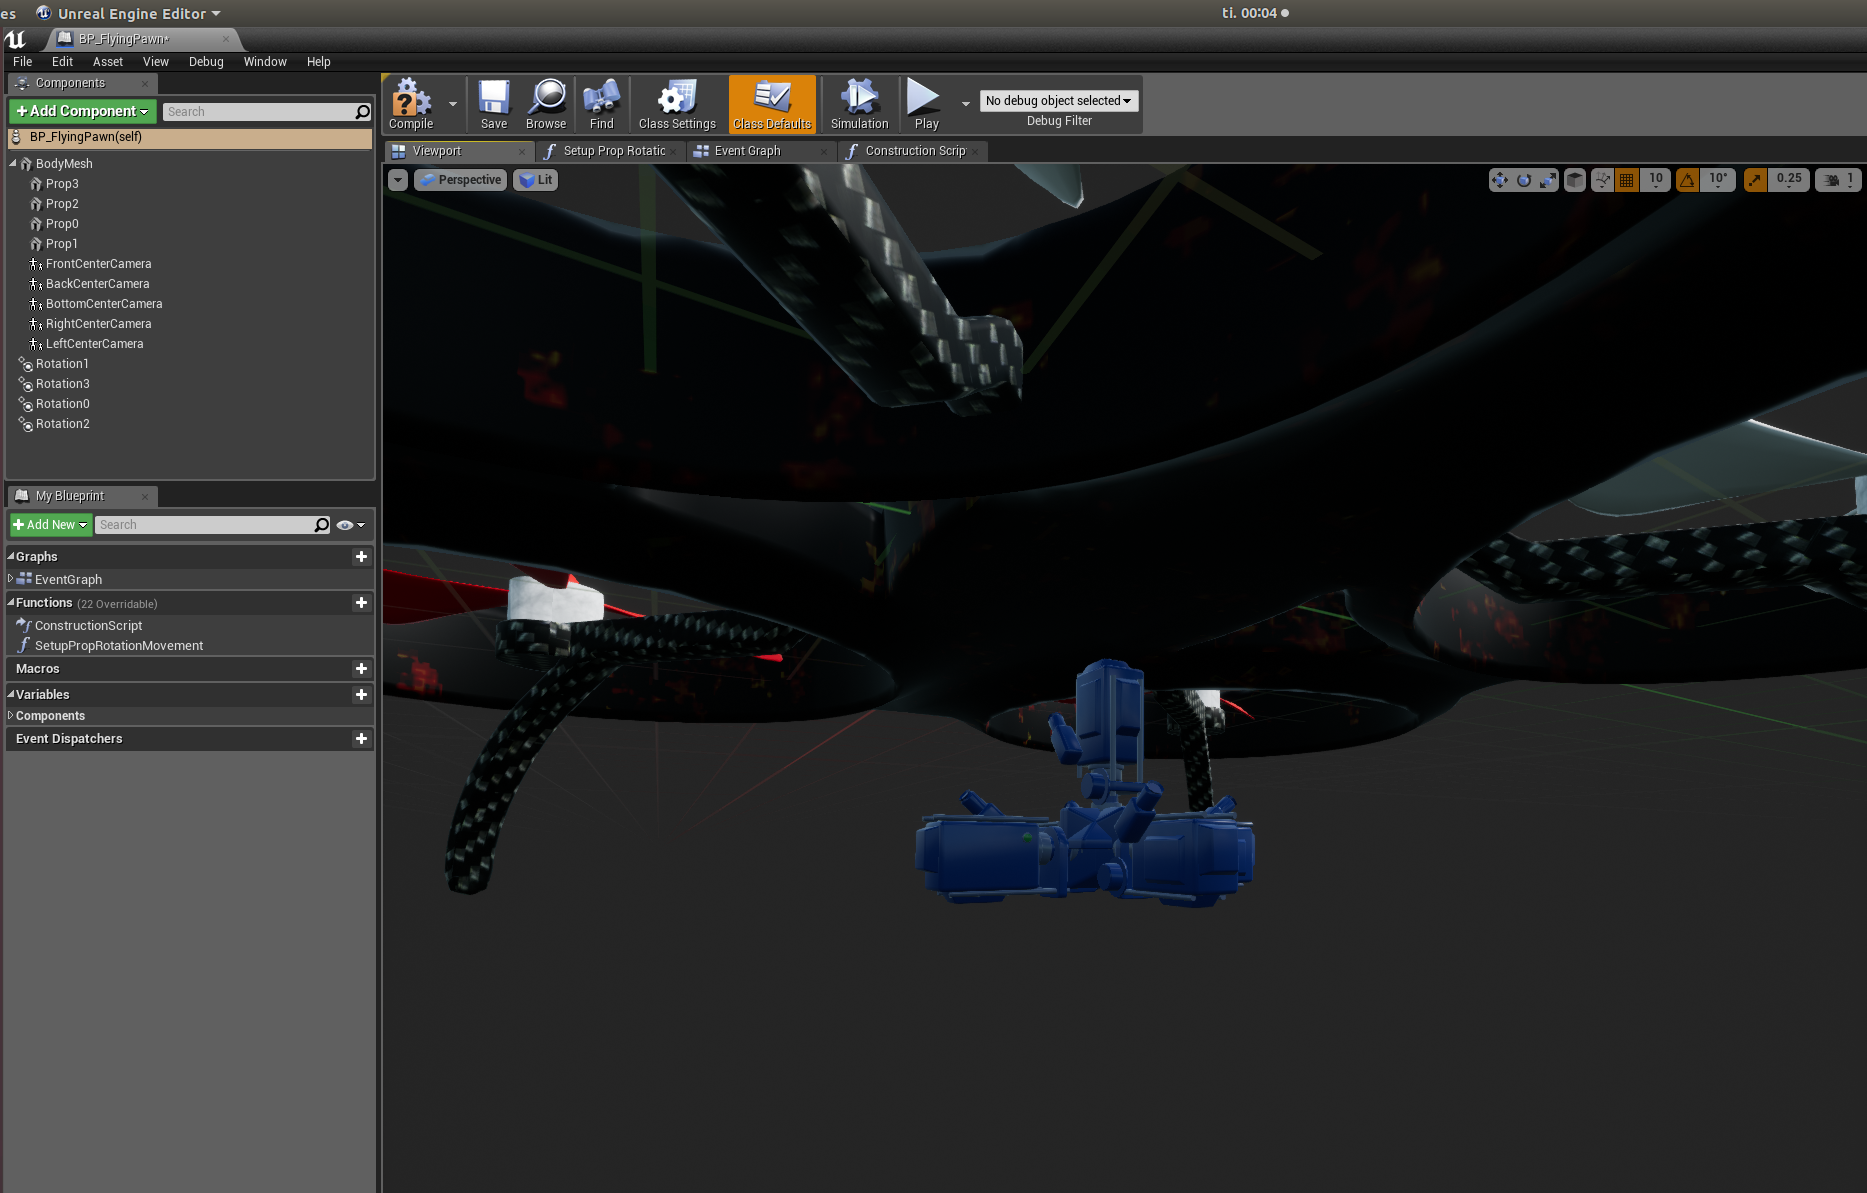
\includegraphics[height=4cm]{rapport/fig/Simulator/camera_setup.png}
        \caption{Fisheye camera setup}
        \label{fig:new_Blueprint_cameras}
    \end{subfigure}
    \begin{subfigure}{0.45\linewidth}
        \centering
        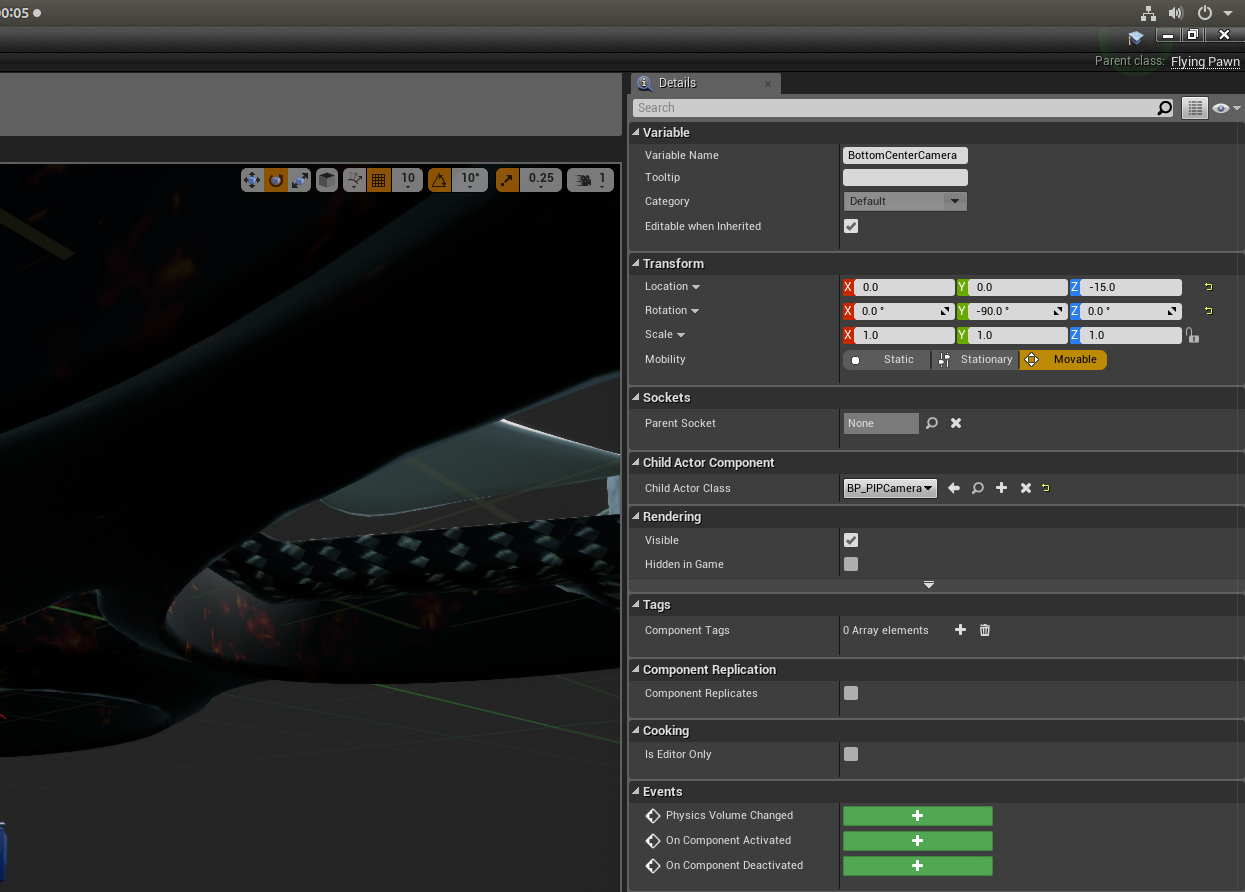
\includegraphics[height=4cm]{rapport/fig/Simulator/camera_setting.png}
        \caption{Downward camera settings}
        \label{fig:new_Blueprint_nodes}
    \end{subfigure}
    \caption{Multirotor Blueprint setup for the fisheye camera, consisting of 5 clustered perspective cameras.}
    \label{fig:new_Blueprint_multirotor}
\end{figure}

\subsection{Projection model}

In order to capture as much as possible of the scene, the far end clipping plane distance was kept at the end of the simulated scene. This is approximated by letting $d_f \rightarrow \infty$ in the perspective projection matrix. AirSim implements Unreal Engines Reversed Perspevtive matrix, which contains the projected volume to be defined by: $x,y \in [-1,1]$ and $z \in [0,1]$. In addition to this, the far clipping plane is projected to $z=0$ and the near clipping plane is projected to $z=1$. Using these constraints and the set of equations in Equation~\eqref{eq:perspective_zeqs} the projection of $Z$ becomes:

\begin{equation}
    \begin{aligned}
        d_n &= Ad_n + B &, for \quad Z &= d_n, z = 1 \\
        0 &= Ad_f + B &, for \quad Z &= d_f, z = 0 \\
        \Rightarrow A &= \frac{d_n}{d_n-d_f} & B &= -\frac{nf}{n-f}
    \end{aligned}
    \label{eq:impl_perspective_zeqs}
\end{equation}

A FoV of $90^\circ$ means that $d_n=1$, since the near clipping plane is defined to be 2 by 2 units wide. Using this as well as letting $d_f \rightarrow \infty$ we get the parameters shown in Equation~\eqref{eq:impl_inf_far_clip}.

\begin{equation}
    \begin{aligned}
    A = \lim_{f \rightarrow \infty} \frac{n}{n-f} =
    \lim_{f \rightarrow \infty} \frac{\frac{n}{f}}{\frac{n}{f}-1} = 
    \frac{0}{-1} = 0 \\
    B = \lim_{f \rightarrow \infty} -\frac{nf}{n-f} = 
    \lim_{ \rightarrow \infty} -\frac{n}{\frac{n}{f}-1} =
    -\frac{n}{-1} = n = 1
    \end{aligned}
    \label{eq:impl_inf_far_clip}
\end{equation}

Adding these to the perspective projection matrix from Equation~\eqref{eq:perspective_projmat_temp}, we get the matrix shown in Equation~\eqref{eq:impl_proj_mat}.

\begin{equation}
    \begin{bmatrix}
        \frac{\rho}{arctan(\Theta/2)} & 0 & 0 & 0 \\
        0 & \frac{1}{arctan(\Theta/2)} & 0 & 0 \\
        0 & 0 & A & B \\
        0 & 0 & 1 & 0 
    \end{bmatrix} = \begin{bmatrix}
        \frac{1}{arctan(\theta/2)} & 0 & 0 & 0 \\
        0 & \frac{1}{arctan(\Theta/2)} & 0 & 0 \\
        0 & 0 & 0 & 1 \\
        0 & 0 & 1 & 0 
    \end{bmatrix}
    \label{eq:impl_proj_mat}
\end{equation}

\subsection{Combining pictures and adding distortion}

Figure~\ref{fig:impl_Sphere_projection} shows the setup for the custom cube capture used by the fisheye camera. The available information through at the client side is the image request response from AirSim. This structure contains: Camera name, Camera position and orientation, time stamp, the picture dimension in pixels, the image type and the image itself. It also contains whether the picture is in PNG format. However, all requests sent to get a fisheye pictures will request a raw RGBA8 picture, so this field is irrelevant. 

\begin{figure}[!htb]
    \centering
    \tdplotsetmaincoords{70}{160}
    \begin{tikzpicture}[tdplot_main_coords, scale = 1.4]
    
    \coordinate (O) at (0,0,0);
    \tdplotsetrotatedcoords{0}{-90}{90}
    
    \coordinate (IMBOTC) at (0,0,-2);
    \tdplotsetrotatedcoordsorigin{(IMBOTC)}
    \draw[tdplot_rotated_coords, thick, fill=black!3, opacity=0.5] (2,0,2) -- (2,0,-2) -- (-2,0,-2) -- (-2,0,2) -- cycle;
    
    \coordinate (IMLEFT) at (0,-2,0);
    \tdplotsetrotatedcoordsorigin{(IMLEFT)}
    \draw[tdplot_rotated_coords, thick, fill=black!3, opacity=0.5] (0,2,2) -- (0,-2,2) -- (0,-2,-2) -- (0,2,-2) -- cycle;
    
    
    \tdplotsetrotatedcoordsorigin{(O)}
    
    \draw[tdplot_rotated_coords, ->] (0,0,2) -- (0,0,3) node[below]{$Z$};
    
    \tdplotsetcoord{IMGC}{2}{-90}{0}
    \tdplotsetrotatedcoordsorigin{(IMGC)}
    \draw[thick, tdplot_rotated_coords, fill=black!2, opacity=0.8] (-2,-2,0) -- (-2,2,0) -- (2,2,0) -- (2,-2,0) -- cycle;
    
    \draw[tdplot_rotated_coords, dashed] (0,0,-1.5) -- (0,0,0);
    
    \draw[tdplot_rotated_coords, dashed, opacity=0.8] (0,0,-2) -- (0,-2,0);
    \draw[tdplot_rotated_coords, dashed, opacity=0.8] (0,0,-2) -- (2,0,0);
    \draw[tdplot_rotated_coords, dashed, opacity=0.8] (0,0,-2) -- (2,2,0);
    \draw[tdplot_rotated_coords, dashed, opacity=0.8] (0,0,-2) -- (2,-2,0);
    \draw[tdplot_rotated_coords, dashed, opacity=0.8] (0,0,-2) -- (-2,-2,0);
    
    \tdplotsetrotatedcoordsorigin{(O)}
    \tdplotsetrotatedcoords{90}{70}{0}
    \draw[tdplot_rotated_coords, thick, fill=black!5, opacity = 0.8] (0:2) arc (0:180:2);
    \tdplotsetrotatedcoords{0}{-90}{90}
    \draw[thick, tdplot_rotated_coords, fill=black!3] (0:2) arc (0:360:2);
    
    \tdplotsetrotatedcoords{0}{-90}{90}
    \draw[tdplot_rotated_coords, ->] (-0.5,0,0) -- (3,0,0) node[below]{$X$};
    \draw[tdplot_rotated_coords, ->] (0,-0.5,0) -- (0,2.5,0) node[right]{$Y$};
    \draw[tdplot_rotated_coords, dashed] (0,0,0) -- (0,0,0.6);
    
    \draw[tdplot_rotated_coords, dashed, opacity=0.8] (1.155,1.155,1.155) -- (2,2,2);
    \draw[tdplot_rotated_coords, dashed, opacity=0.8] (1.155,0,1.155) -- (2,0,2);
    \draw[tdplot_rotated_coords, dashed, opacity=0.8] (1.155,-1.155,1.155) -- (2,-2,2);
    
    \draw[tdplot_rotated_coords, dashed, opacity=0.8] (0,0,0) -- (0.5,0.5,0.5);
    \draw[tdplot_rotated_coords, dashed, opacity=0.8] (0,0,0) -- (0.5,0,0.5);
    \draw[tdplot_rotated_coords, dashed, opacity=0.8] (0,0,0) -- (0.5,-0.5,0.5);
    \draw[tdplot_rotated_coords, dashed, opacity=0.8] (0,0,0) -- (0,-0.6,0.6);
    \draw[tdplot_rotated_coords, dashed, opacity=0.8] (0,0,0) -- (-0.7,-0.7,0.7);
    
    
    \tdplotsetcoord{IMTOPC}{2}{0}{-90}
    \tdplotsetrotatedcoordsorigin{(IMTOPC)}
    \draw[tdplot_rotated_coords, thick, fill=black!2, opacity=0.5] (2,0,2) -- (2,0,-2) -- (-2,0,-2) -- (-2,0,2) -- cycle;
    \end{tikzpicture}
    
    \caption{Projection from perspective camera to a unit sphere using 5 perspective cameras, given a FoV of $180^\circ$. Image plane at $X=1$ is not shown.}
    \label{fig:impl_Sphere_projection}
\end{figure}

To provide a correct projection, the angles $\phi$ and $\theta$, shown in Figure~\ref{fig:fisheye_spherical_projection} must be known. In order to convert the pixel positions to these angles, it is beneficial to change to image coordinates on a plane with $x^i,y^i \in [-1,1]$. Here $[x^i, y^i]^\top$ and $u^i,v^i]^\top$ refer to the image and pixel coordinates on the intermediate image plane, not to be confused with $[x, y]^\top$ and $[u^i,v^i]^\top$, which are the image and pixel coordinates of the fisheye picture. With the aspect ratio $\rho = 1$, each perspective image will be of dimention $W \times H = W \times W$ pixels. Using this and the matrix from Equation~\eqref{eq:pixel_transform}, we get Equation~\eqref{eq:impl_pixel_inverse_transform}:

\begin{equation}
    \begin{bmatrix}
        x^i \\ y^i \\ 1
    \end{bmatrix} = \begin{bmatrix}
        \frac{W}{2} & 0 & u_0 \\
        0 & \frac{H}{2} & v_0 \\
        0 & 0 & 1
    \end{bmatrix}^{-1}\begin{bmatrix}
        u^i \\ v^i \\ 1
    \end{bmatrix} = \begin{bmatrix}
        \frac{2}{W} & 0 & -1 \\
        0 & \frac{2}{W} & -1 \\
        0 & 0 & 1
    \end{bmatrix}\begin{bmatrix}
        u^i \\ v^i \\ 1
    \end{bmatrix}
    \label{eq:impl_pixel_inverse_transform}
\end{equation}

As of now, the image coordinates are represented in their local coordinate frame. However, by design the downward pointing camera defines the forward direction of the camera, hereforth named with the superscript $\{\}^d$. Hence, all image coordiantes needs to be rotated to this frame. AirSim provides a library for quaternion math, which will be used for this conversion. Table~\ref{tab:impl_quaternion_rotations} show the respective quaternion rotations for the named cameras:

\begin{table}[!htb]
    \centering
    \begin{tabular}{|c|c|c|c|} \hline
        $p^i$ & Camera Direction & $R^d_i = R_{x,\psi}(\psi)R_{y,\eta}(\eta)$ & Quaternion $q_{d,i}$ \\ \hline \hline
        $p^d$ & Down & 0, 0 & $[1,0,0,0]^\top$ \\ \hline
        $p^f$ & Front & 0, -90 & $[0.707,0,0.707,0]^\top$ \\ \hline
        $p^r$ & Right & -90, -90 & $[0.5,-0.5,-0.5,-0.5]^\top$\\ \hline
        $p^b$ & Back & 180, -90 & $[0,0.707,0,0.707]^\top$ \\ \hline
        $p^l$ & Left & 90, -90 & $[0.5,0.5,-0.5,0.5]^\top$\\ \hline
    \end{tabular}
    \caption{Rotation needed to rotate image coordinate $x^i$ to $x^d$}
    \label{tab:impl_quaternion_rotations}
\end{table}

Allplying the rotation, alongside Equation~\eqref{theory_polar_coords}, using $[X,Y,Z]^\top=[x^d,y^d,z^d]^\top$, we get the following angles $\phi$ and $\theta$, seen in Equation~\eqref{eq:impl_polar_transform}, which are implemented using the atan2 function from the standard library.

\begin{subequations}
    \begin{equation}
        p^d = \begin{bmatrix} x^d \\ y_d \\ z_d \end{bmatrix} = q_{d,i} p^i q_{d,i}^\top
        \label{eq:impl_polar_transform_quaternion}
    \end{equation}
    \begin{equation}
        \theta = arctan\left(\frac{y^d}{x^d}\right)
        \label{eq:impl_polar_transform_theta}
    \end{equation}
    \begin{equation}
        \phi = arccos\left(\frac{z^d}{\sqrt{(x^d)^2 + (y^d)^2 + (z^d})^2}\right) = arctan\left(\frac{\sqrt{(x^d)^2 + (y^d)^2}}{z^d}\right)
        \label{eq:impl_polar_transform_phi}
    \end{equation}
    \label{eq:impl_polar_transform}
\end{subequations}


The camera lens is implemented with the polynomial model presented in Table~11.1 in \cite{FisheyeCorke}. For now this is implemented as a fourth order polynomial:

\begin{equation}
    r(\phi) = k_1 \phi + k_2 \phi^2 + k_3 \phi^3 + k_4 \phi^4
    \label{eq:impl_lens_model}
\end{equation}

Here This allows for a quite flexible distortion model. For example the equiangular model described in Equation~\eqref{eq:fisheye_to_image} is found by setting $k_1 = f$, $k_2 = k_3 = k_4 = 0$. It can be seen from Equation~\eqref{eq:impl_lens_model} that the resolution of must be controlled by:

\begin{equation}
    \begin{aligned}
        u_{max} = v_{max} &> ||k_1 \phi_{max} + k_2 \phi_{max}^2 + k_3 \phi_{max}^3 + k_4 \phi_{max}^4 ||_2 \\
        &= || 135k_1 + 135^2 k_2 + 135^3 k_3 + 135^4 k_4 ||_2 \\
        &= \sqrt{(135k_1)^2 + (135^2 k_2)^2 + (135^3 k_3)^2 + (135^4 k_4)^2} \\
        &< 332.159.737,9 \quad, for \quad k_1,k_2,k_3,k_4 \leq 1 
    \end{aligned}
    \label{eq:impl_size_criteria}
\end{equation}

All numbers integers may be stored within a long int (64 bit) and a double variable will be used for the lens parameters. The upper limit will be set to 1 for the parameters, making sure that the module is able to store the numbers in one variable. While the output picture resolution will be computed and satisfy Equation~\eqref{eq:impl_size_criteria}, it is important to calibrate these parameters according to you own camera. Most likely, $k_1$ will be dominant, as it holds the normal radial distortion.

\subsection{ROS interface to AirSim and fisheye camera}\label{subsec:ROS_interface}

The ROS interface is split into two different parts: The first part handles AirSim ImageRequests, and the fisheye transformations, while the other handles ROS publishing. The package inherits the base RPC-Client API class defined for AirSim, and does by itself only depend on the client base API implementation, and of course ROS, to create a link between the two. However, for the added functionality of publishing fisheye images, it also depends on the fisheye module, OpenCV and cv\_bridge\footnote{https://github.com/ros-perception/vision\_opencv}. Where cv\_bridge handles the conversion between the OpenCV image object and the ROS image message.

Using the custom setup discussed in Section~\ref{subsec:Fisheye_impl_overview}, the requests for the perspective images are treated by referencing the cameras by name. As of this moment, I have not found a better way to do this, as the AirSim API does not implement polling for available cameras. The received vector of images is then converted to OpenCV images and wrapped into a custom FisheyeImageRequest made for this project. This structure holds the images, image size, and information about the camera pose, which is necessary to compute the final image.

The created ROS node runs an infinite loop, shown in Figure~\ref{fig:impl_ROS_pub_loop}. The loop is interruptable by crtl+c through the ros::ok() function. The loop consists of polling for images, conversion to fisheye image, and publishing the image on the FisheyImage ROS topic. The complete implementation of the ROS interface is unfortunately not finished, meaning that in order to control the multirotor, the old client API needs to be included and used in the client application. Both the ROS publisher and the old client API can be run simultaneously.

\begin{figure}[!htb]
    \centering
    \begin{tikzpicture}[node distance=2cm, transform shape, scale=0.7]
        \tikzstyle{start} = [rectangle, rounded corners, minimum width = 2cm, minimum height = 1cm, text centered, draw=black, fill=red!10]
        \tikzstyle{if} = [diamond, minimum width = 2.5cm, minimum height = 1.5cm, text centered, draw=black, fill=blue!10]
        \tikzstyle{task} = [rectangle, rounded corners, minimum width = 3cm, minimum height = 1.5cm, text centered, draw=black, fill=blue!10]
        \tikzstyle{singlearrow} = [thick, ->, >=stealth]
        
        \node (START) [start]{Start};
        \node (CONN) [task, below of=START, align=center, yshift=0.45cm]{Connect to \\ mutlirotor};
        \node (PUBINIT) [task, below of=CONN, align=center]{Initialize \\ Publisher};
        
        \node (ROSOK) [if, below of=PUBINIT, yshift=-0.8cm]{ros::ok()?};
        \draw[] (ROSOK) node[xshift=1.7cm, yshift=0.3cm]{yes};
        \draw[] (ROSOK) node[xshift=0.5cm, yshift=-1.5cm]{no};
        \node (REQ) [task, align=center, right of=ROSOK, xshift=1.7cm]{Request \\ Images};
        \node (OPENCV) [task, align=center, right of=REQ, xshift=1.3cm]{Convert to \\ cv::Mat};
        \node (FISH) [task, align=center, right of=OPENCV, xshift=1.3cm]{Create \\ fisheye image};
        \node (CONV) [task, align=center, right of=FISH, xshift=1.75cm]{Convert to ROS \\ sensor\_msgs/Image};
        \node (PUB) [task, align=center, right of=CONV, xshift=1.75cm]{Publish to \\ /FisheyeImage};
        
        \node (DISC) [task, align=center, below of=ROSOK, yshift=-0.5cm]{Disconnect from \\ multirotor};
        \node (END) [start, below of=DISC, yshift=0.45cm]{End};
        
        \draw[singlearrow] (START) -- (CONN);
        \draw[singlearrow] (CONN) -- (PUBINIT);
        \draw[singlearrow] (PUBINIT) -- (ROSOK);
        \draw[singlearrow] (ROSOK) -- (REQ);
        \draw[singlearrow] (REQ) -- (OPENCV);
        \draw[singlearrow] (OPENCV) -- (FISH);
        \draw[singlearrow] (FISH) -- (CONV);
        \draw[singlearrow] (CONV) -- (PUB);
        \path[draw, -latex, singlearrow] (PUB) -- ++(0cm,1.7cm) -| (ROSOK);
        \draw[singlearrow] (ROSOK) -- (DISC);
        \draw[singlearrow] (DISC) -- (END);
        
    \end{tikzpicture}
    \caption{ROS publisher loop}
    \label{fig:impl_ROS_pub_loop}
\end{figure}




\cleardoublepage